\documentclass{article}
\usepackage{spconf,amsmath,epsfig}
\usepackage[utf8]{inputenc}
\usepackage{graphicx}
\usepackage{verbatim}

% autoref command
\usepackage[pdftex,urlcolor=black,colorlinks=true,linkcolor=black,citecolor=black]{hyperref}
\def\sectionautorefname{Section}
\def\subsectionautorefname{Subsection}
\def\figureautorefname{Fig.}
\def\subfigureautorefname{Fig.}

\title{DEFINING AESTHETIC PRINCIPLES FOR AUTOMATIC MEDIA GALLERY LAYOUT\\
FOR VISUAL AND AUDIAL EVENT SUMMARIZATION BASED ON SOCIAL NETWORKS}

\twoauthors
  {Thomas Steiner$^1$, Ruben Verborgh$^2$}
	{$^1$Universitat Politècnica de Catalunya\\
	Llenguatges i Sistemes Informàtics (LSI)\\
	08034 Barcelona, Spain\\
	\texttt{tsteiner@lsi.upc.edu},\\
	\texttt{gabarro@lsi.upc.edu}}
  	{Joaquim Gabarro$^1$, Rik Van de Walle$^2$}
	{$^2$Ghent University -- IBBT,\\
	ELIS -- Multimedia Lab,\\
	B-9050 Ledeberg-Ghent, Belgium\\
	\texttt{ruben.verborgh@ugent.be},\\
	\texttt{rik.vandewalle@ugent.be}}

\let\oldsection\section
\renewcommand{\section}[1]{\oldsection{#1}\vspace{-1em}}
\hyphenation{visual exploited}

\begin{document}

\maketitle

\begin{abstract}
In this paper, we present and define aesthetic principles
for the automatic generation of media galleries
based on media items retrieved from social networks
that---after a ranking and pruning step---can serve to authentically
summarize events and their atmosphere from a visual
and an audial standpoint.
\end{abstract}

\begin{keywords}
event summarization, media galleries, social networks,
media item ranking, media layout, aesthetics
\end{keywords}

\vspace{-0.4em}
\section{Introduction}
Mobile devices such as smartphones, together with social networks,
enable people to create, share, and consume media items
like videos or images.
They accompany their owners almost everywhere
and are thus omnipresent at all sorts of events.
Given a~stable network connection, event-related media items
and microposts are published on social networks
during events and afterwards.
Ranked media items stemming from multiple social networks
can serve to create authentic media galleries
that illustrate events and their atmosphere.
A~key feature for this task is the semantic enrichment
of media items and associated microposts
and the extraction of \textbf{visual}, \textbf{audial},
\textbf{textual}, and \textbf{social} features.
Based on this set of features,
additional \textbf{aesthetic} features
can be defined and exploited to obtain appealing
and harmonic media galleries.
% RV: How to extract aesthetic features? Aren't aesthetics part of the visual, audial, and textual components?
% TS: Added an additional sentence to clarify.

\begin{comment}
\begin{figure}[htb]
\centering
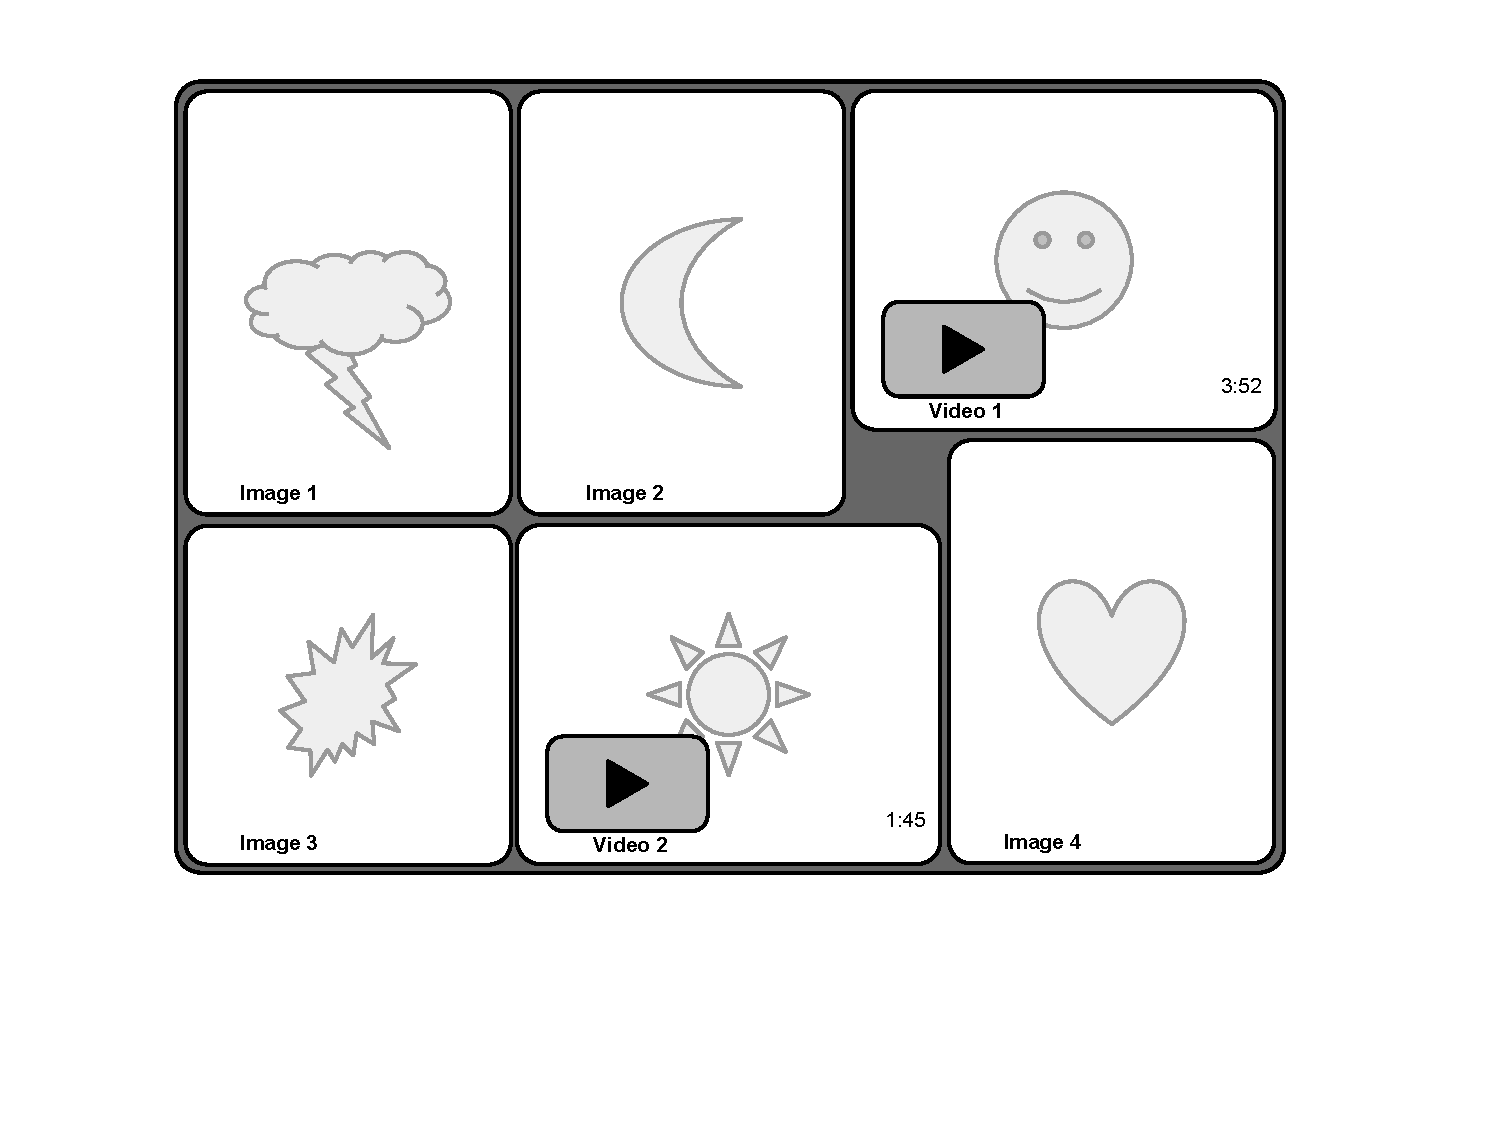
\includegraphics[trim=20mm 40mm 20mm 10mm, clip, width=0.75\columnwidth]{media-gallery.pdf}
\caption{Schematic media gallery with 4 images and 2 videos.}
\label{fig:media-gallery}
\end{figure}
\end{comment}

\vspace{-0.4em}
\section{Related Work}
While enormous efforts have been made to extract those features
from media items and microposts on social networks in \emph{isolation},
to the best knowledge of the authors, remarkably less initiatives 
concern the extraction and the application
of all those features \emph{in combination}
for \emph{all} types of media items, including microposts.
In~\cite{Photo2011}, Sandhaus \emph{et al.}\ consider visual and
aesthetic features for the automatic creation of photo books.
Obrador \emph{et al.}\ use visual and aesthetic features
for a category-based approach to automatically assess
the aesthetic appeal of photographs~\cite{Photo2012}.
In~\cite{Playlist2006}, Knees \emph{et al.}\ use audial and textual
features for the automatic generation of music playlists.
Choudhury \emph{et al.}\ show in \cite{Sports2011} how social and textual
features can be used to achieve precise detection results 
of named entities and significant events in sports-related microposts.
In~\cite{YouTube2010}, Davidson \emph{et al.}\ show how visual,
textual, and social features can be used for personalized video recommendations.
A service called Storify~\cite{Storify2011} lets users manually combine
microposts, images, videos, and other elements onto one page for the purpose
of storytelling or summarizing an event,
and share stories permanently on the Web.
Finally, social networks present images and videos
often in grid-like galleries\footnote{\url{http://twitpic.com/904yka/full}}, sometimes scaled
based on the amount of comments.

\vspace{-0.4em}
\section{Media Item Ranking Criteria}
In this section, we describe several feature categories that can serve to rank
media items retrieved from social networks. 
We assume (and are working on) media item extractors that,
given event-related search terms,
extract raw binary media items and associated microposts
from multiple social networks.

\noindent \textbf{Visual}
This category regards the contents of images and videos.
We distinguish \emph{low-} and \emph{high-level} visual ranking criteria.
High-level criteria are, \emph{e.g.}, logo detection,
face recognition, and camera shot separation.
Low-level criteria are, \emph{e.g.}, size, resolution,
duration, geolocation, and time.
Via OCR, contained characters can be treated as textual features.

\noindent \textbf{Audial}
This category regards the audio track of videos.
\emph{High-level} ranking criteria are the presence or absence
of silence, music, speech, or a mixture thereof.
Similar to visual features before,
audial \emph{low-level} features are the average bit rate,
volume, possibly distorted areas, \emph{etc}.
Through audio-transcription, speech can be converted to a textual feature.

\noindent \textbf{Textual}
This category regards the microposts that accompany media items.
Typically, microposts provide a~description of media items.
Using named entity disambiguation tools,
textual content can be linked to LOD cloud concepts~\cite{Facebook2011}.

\noindent \textbf{Social}
This category regards social network effects like shares, mentions,
view counts, expressions of (dis)likes, user diversity, \emph{etc}.
Prior work~\cite{RAMSS2012} allows us to not only examine these effects
on a~\emph{single} social network,
but in a~\emph{network-agnostic} way across multiple social networks.
% RV: Damn, I'd want a reference for "previous work", but we're running out of space.
% An option is to typeset references in small (and to undo the vspace fix I did that currently shortens the paper length).
% TS: The problem is that the ICMR paper was rejected. 

\noindent \textbf{Aesthetic}
This category regards the desired outcome after the ranking, \emph{i.e.},
the media gallery that illustrates a given event and its atmosphere.
Studies exist for the aesthetics of
automatic photo book layout~\cite{Photo2011},
photo aesthetics \emph{per se}~\cite{Photo2012},
video and music playlist generation~\cite{YouTube2010,Playlist2006},
however media gallery composition requires mixing video
\emph{and} image media items.
% RV: Now it becomes indeed clear that aesthetics is not an extracted feature, but a post-factum criterium, right?
% TS: Hopefully.

\vspace{-0.4em}
\section{Media Gallery Aesthetics}

\noindent \textbf{Definition}
A media gallery in our context is a compilation of images or videos
retrieved from social networks that are related to a given event.
Given a set $M = \{m_1,..., m_n\}$ of media items related to a certain event,
and given a ranking formula $f$,
the subset $M^\prime \subset M$
is the result after the application of $f$ to $M$: $f(M)=M^\prime$.
Each media item $m_i$ can either be an instance of video or image.
For each point $t_x$ on a timeline $T$, the state of the media gallery
at $t_x$ is defined for each media item $m_i$
as a set $S_x$ of $n$ tuples $s_{x,i}$, where
$s_{x,i}=\langle \mathit{left}$, $\mathit{top}$, $\mathit{width}$, $\mathit{height}$,
$\mathit{alpha}$, $\mathit{z\mbox{-}index}$, $\mathit{animation}$,
$\mathit{start}$, $\mathit{playing}$, $\mathit{volume} \rangle$.
The first 6~properties are defined as in CSS, the $\mathit{animation}$ property
allows for the definition of CSS transitions
and transformations as defined in~\cite{CSSTransitions2009,CSSTransforms2012},
the $\mathit{start}$ property defines the start time in a video.
A schematic media gallery at $t_x$ can be seen online\footnote{\url{http://twitpic.com/9je27h/full}}.

\noindent \textbf{Audial aesthetics}
We recall the purpose of our media galleries:
to illustrate an event and its atmosphere.
Audial aesthetics thus consist of aspects like volume level normalization,
avoiding multiple videos playing music in parallel, smooth transitions, \emph{etc}.
We remark that through selective mixing of audio tracks
of event-related videos, ``noise clouds'' very characteristic
for the event atmosphere can be observed.

\noindent \textbf{Visual aesthetics}
Visual aesthetics are determined by the composition, \emph{i.e.},
the relation of images to videos \emph{globally}, \emph{per coherent scene},
and per \emph{point in time}.
In order not to overcharge the perceptive capacity
of viewers, the number of visible (moving) media items
at a time should be limited.
Depending on the event, a consistent or a contrasty overall
appearance of items may be desired, also for transitions.

\vspace{-0.4em}
\section{Preliminary Results and Conclusion}
We have introduced media item ranking criteria and
aesthetic audial and visual principles for media galleries
and, during first experiments, have manually evaluated them
with positive results on a~set of images and videos
that were collected for events in recent history
(among others the \textit{Costa Concordia} disaster in Italy,
the \textit{Consumer Electronics Show} in Las Vegas,
the global \textit{Blackout SOPA} campaign).
Especially when combining mixed content, \emph{i.e.}, videos and images,
users expressed they preferred images and videos to crossfade smoothly 
rather than having sharp contrasts between transitions.
In consequence, we will put special emphasis on shot detection with video content
to ensure a~harmonic holistic perception of mixed content in media galleries.
In the coming months, we will apply those principles
to a large collection of media items related to events,
and, via automatic multivariate blind tests, measure user engagement
for different feature configurations on both desktop and mobile.

% decrease space between bibliographic references
\let\oldbibitem\bibitem
\renewcommand{\bibitem}[1]{%
	\ifx\bibstarted\undefined
		\def\bibstarted{1}
		\vspace{.1em}
	\else
		\vspace{-.2em plus .1em minus .1em}
	\fi
\oldbibitem{#1}}

\bibliographystyle{IEEEbib}
\bibliography{steiner.bib}

\end{document}
